\documentclass[titlepage]{article}
\usepackage{fullpage}
\usepackage{graphicx}

\begin{document}

\title{17-614 Formal Methods\\[1ex] Project: Structural Modeling}
\author{
	{\Large\textbf{Team 16}}\\[3ex]
	yashanan\\[1ex] salonisi\\[1ex] halkhala\\[1ex] ktakayam}
\date{\today}
\maketitle

\newpage

\section{Task 1}
\subsection{Include an object model diagram for your system.}

Below is the final version of our object model diagram. Note that the privacy levels in the below model are singleton sets, so we have used rounded corners to represent them.

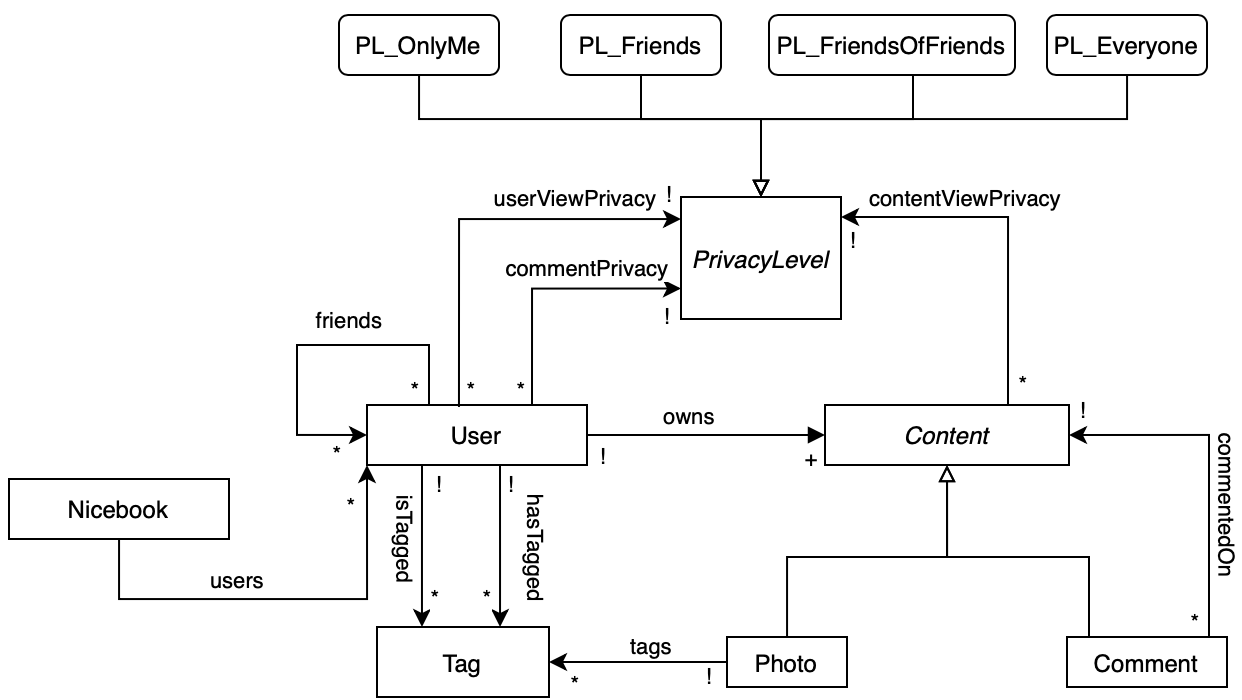
\includegraphics[width=6in]{images/single_model.png}

However, this model holds true only for a ‘snapshot’ of a single Nicebook. Below is the true model (that always holds), where we have redefined some object constraints to accommodate multiple Nicebook situations that arise when modeling actions (see section II.2.2). For e.g., some Content can be owned by two different users, given that they belong to different Nicebooks - a situation that arises during addPhoto when we need to copy a User to preserve all their existing Content.

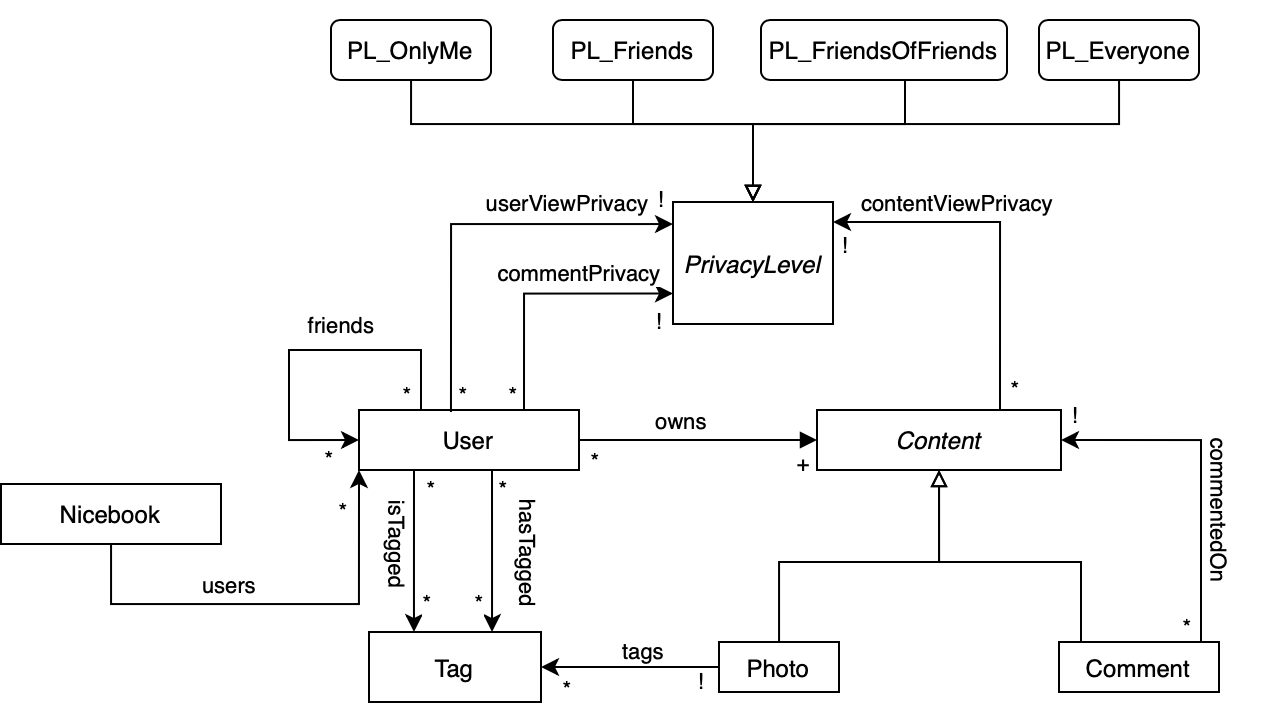
\includegraphics[width=6in]{images/true_model.png}

\subsection{Describe any decisions that your team made in resolving ambiguities in the English document. Also describe alternatives you considered and rejected.}

The decisions we made during the modeling process fall roughly into two categories: “Feature decisions” and “Internal modeling decisions”.
\subsubsection{Feature Decisions}
These are decisions we made regarding features that are exposed to the users.
\begin{enumerate}
\item\textbf{Privacy Settings}\\
There are three types of privacy settings defined in the project specification:
\begin{enumerate}
	\item Each piece of content owned by a user is associated with a privacy level that determines who can view that content on the user’s account.
	      \begin{enumerate}
		      \item We have defined a relationship contentViewPrivacy: Content $\rightarrow$ PrivacyLevel which is a content-specific setting that controls who related to the user can view user-owned content.
	      \end{enumerate}
	\item Each user has a setting that controls who can view content that is published on the user’s account by other users.
	      \begin{enumerate}
		      \item We assume that comments posted (both direct and nested) on user-owned content are considered content published by other users on the user’s account.
		      \item We have defined a relationship userViewPrivacy: User $\rightarrow$ PrivacyLevel which is a user-specific setting that controls viewing privileges for comments attached to user-owned content.
	      \end{enumerate}
	\item Each user has a setting that controls who can add a comment to content that is owned by the user.
	      \begin{enumerate}
		      \item We have defined a relationship commentPrivacy: User $\rightarrow$ PrivacyLevel which is a user-specific setting that controls who can comment on user-owned content.
	      \end{enumerate}
\end{enumerate}
\item\textbf{Content Viewing Priveleges}
\begin{enumerate}
	\item The $getContentsInState[s: Nicebook]$ function returns the set of Content that belongs to the state s. A Content instance belongs to a state if the owner of the content as well as the owners of all parent contents (if any) belong to the state. In the below example, Comment belongs to S1 in the left state-chart since its user as well as the owner of its parent Content (Photo) belong to the state S1. However, in the right diagram, the owner of Comment belongs to S1, but since the owner of its parent Content does not belong to S2, Comment does not belong to S1 in the right diagram.

	      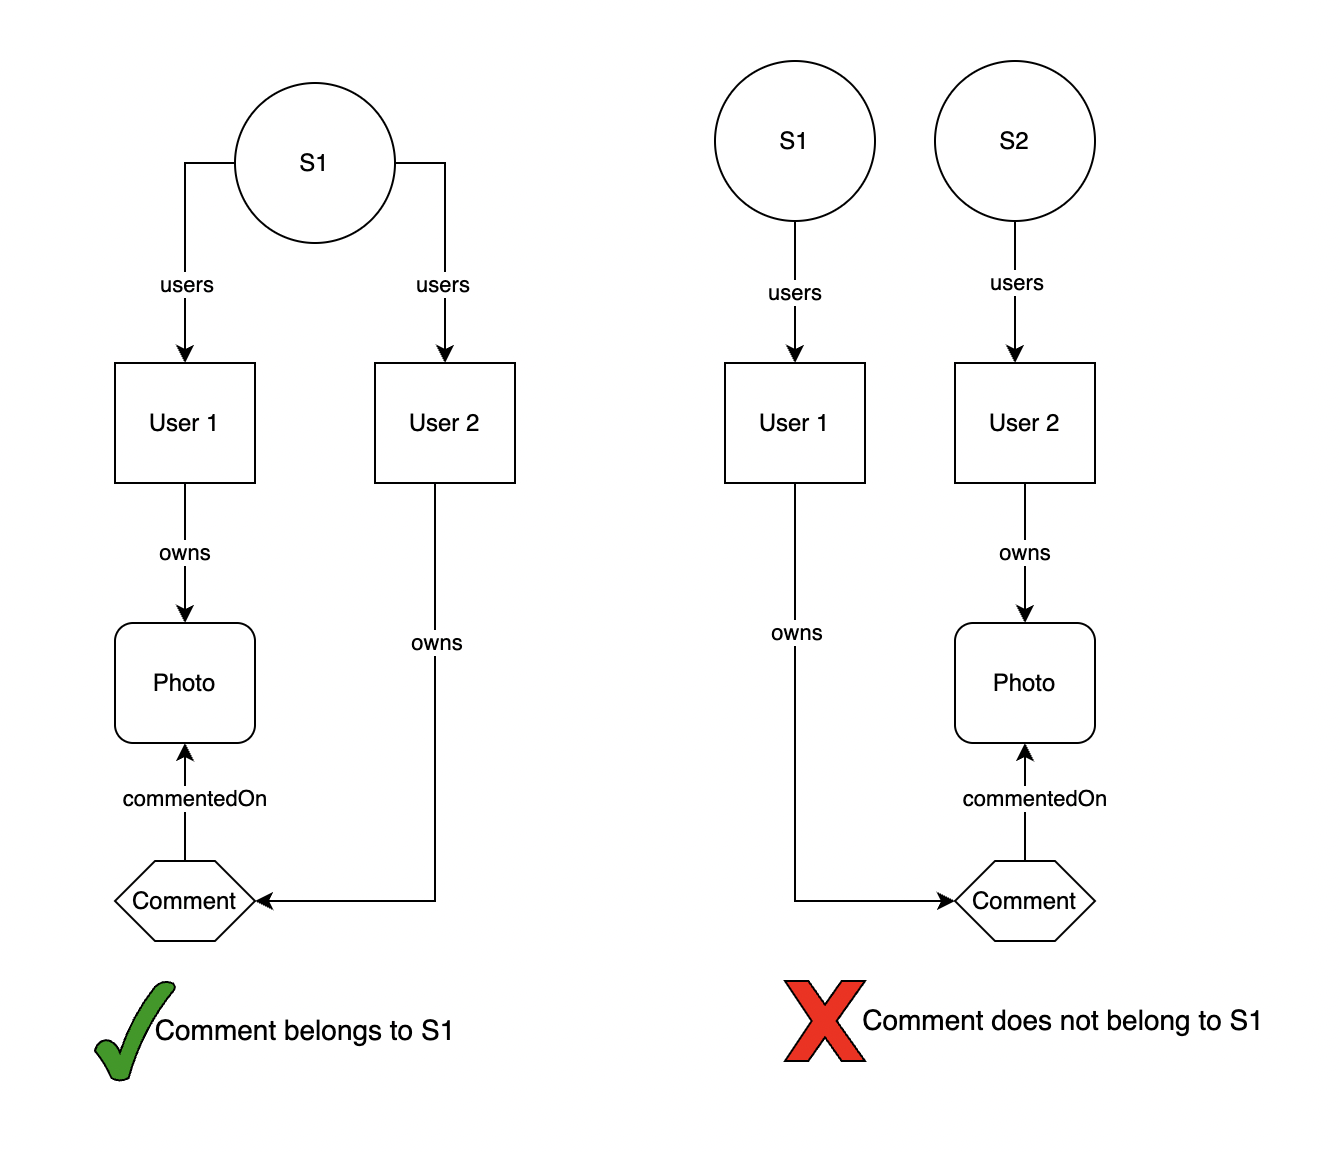
\includegraphics[width=6in]{images/content_view_1.png}

	\item We have defined a function called $canView$ which takes a User instance and a Nicebook instance (representing the state) as arguments and returns the set of Contents that the user can view in a given state. A user can view Content if all of the following conditions hold:

	      \begin{enumerate}
		      \item The content belongs to the state
		      \item The user has viewing privileges for the said content as defined in the $contentViewPrivacy$ relation.
		      \item If the user has parent elements, the user must have privileges to view the “children” elements of parent elements. This is defined in the $userViewPrivacy$ relation.
		      \item All the above conditions must satisfy for the content at hand as well as all parent elements of the said content – In short, a content can only be viewed if all its parent contents can also be viewed.
	      \end{enumerate}
	      \item\textbf{Exception: A user can view all comments and nested comments on content owned by him/her regardless of the contentViewPrivacy and userViewPrivacy settings defined by those comments and owners of those comments respectively.}
\end{enumerate}
\item\textbf{Commenting Priveleges}
\begin{enumerate}
	\item We have defined a function canCommentOn[u: User, s : Nicebook] which returns the set of Contents that the user can comment on. A user can comment on a content if the following conditions hold:
	      \begin{enumerate}
		      \item The user can view the content as defined in the canView function.
		      \item The user has commenting privileges as defined by the content owner in the commentPrivacy relation.

		      \item The above conditions must hold true for all its parent content elements, if any.
	      \end{enumerate}
	      \item\textbf{Exception: A user can comment on comments and nested comments that are attached to contents owned by the user, regardless of the commentPrivacy settings set up by owners of those nested comments.}
	      \item\textbf{Operation Priveleges}
	      \begin{enumerate}
		      \item \underline{Adding a photo}: Any user can perform this action. When a photo is added by a user, the relationship “owns” is established between the user and the photo.
		      \item \underline{Deleting a photo}: A photo can be deleted by the owner of the photo only.
		      \item \underline{Adding a comment}: To add a comment on an instance of Content, the following conditions must hold true:
		            \begin{enumerate}
			            \item The user must have commenting privileges on content as defined in the canCommentOn function.
		            \end{enumerate}
		      \item \underline{Deleting a comment}: In order to delete a comment, either of the following must hold:
		            \begin{enumerate}
			            \item The user is the owner of the comment
			            \item The user is the owner of one of the parent elements of the said comment.
			                  \end {enumerate}
			            \item \underline{Adding a tag}: A user can tag another user on a photo if the following holds true:
			                  \begin{enumerate}
				                  \item Both users have the privilege of viewing the Photo.
				                  \item The two users are friends in the same state
			                  \end{enumerate}
			            \item \underline{Removing a tag}: A user can remove a tag if any one or more of the following conditions holds true:
			                  \begin{enumerate}
				                  \item The user is the owner of the Photo which is tagged.
				                  \item The user is tagged on a Photo and wants to remove his/her own tag from the Photo.
				                  \item The user has tagged another user on a Photo and now wants to remove this tag.
			                  \end{enumerate}
		            \end{enumerate}
	      \end{enumerate}
\end{enumerate}

\subsubsection{Internal Modeling Decisions}
These are internal alloy-related modeling decisions that do not affect what a user sees but how we choose to model our system.
\begin{enumerate}
	\item \textbf{Modeling Tags}\\
	      When it came to modeling tags, we realized that one of the constraints in the spec was to ensure that Users can only tag their friends. We considered three options:
	      \begin{enumerate}
		      \item Define three relationships for Tags, one with the tagged User (taggee), one with the tagger User, and one with the Photo.
		      \item Define a ternary relationship ‘tagging: User $\rightarrow$ User’, and one with the Photo.
		      \item Simply restrict tagging to friends only in the addTag action.
	      \end{enumerate}
	      We found that although option (c) seemed the simplest to implement, we would not be able to constrain our model tightly enough. Alloy would always be able to generate a fresh instance where the constraint is violated because addTag has never happened. Option (b) is a good choice, but we agreed it’s more consistent with the rest of the model if we simply have a separate relation to each User.
	\item \textbf{Modeling Deletion}\\
	      When it comes to deleting some Content, we had two options to choose from:
	      \begin{enumerate}
		      \item For the owner, create a new User in the new Nicebook state, who no longer owns the Content, and additionally ensure that no other user in the new Nicebook has any link to this Content through Comments or Tags. So that there is no way to reach the Content from the new Nicebook state.
		      \item For the owner, create a new User in the new Nicebook state, who no longer owns the Content, but retain all other relationships of this deleted Content, and make it impossible for anyone to view it.
	      \end{enumerate}
	      The problem with option (a) is that to ensure no Users in the new Nicebook state have a link to the deleted Content, we will have to copy every User to the new state. To truly copy these Users, we need to preserve their Friendships too, which cannot be achieved without redefining our signatures or augmenting our current model with additional relationships that allow us to link an ‘old’ state of a User to its ‘future’ state. In the below example, for deleting photo1 we created two new users user1\_new and user2\_new as they were linked in some way to photo1. Since user1\_old and user2\_old were friends we need to ensure user1\_new and user2\_new are also friends.

	      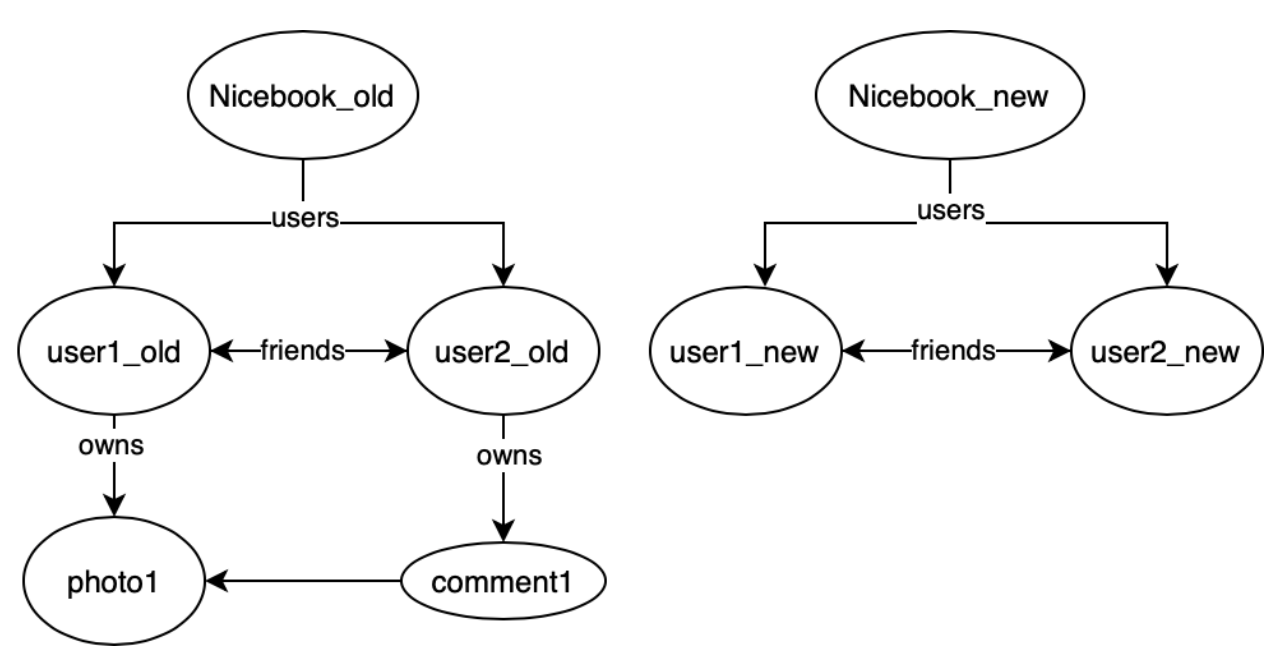
\includegraphics[width=6in]{images/modeling_decision_1.png}

	      Since a User can have any arbitrary number of friends it becomes very difficult (given our signatures) to write a generic predicate that will ensure all the Friendships are retained. We need a new relation, like ‘future’, to link old User states to new ones, as shown below.

	      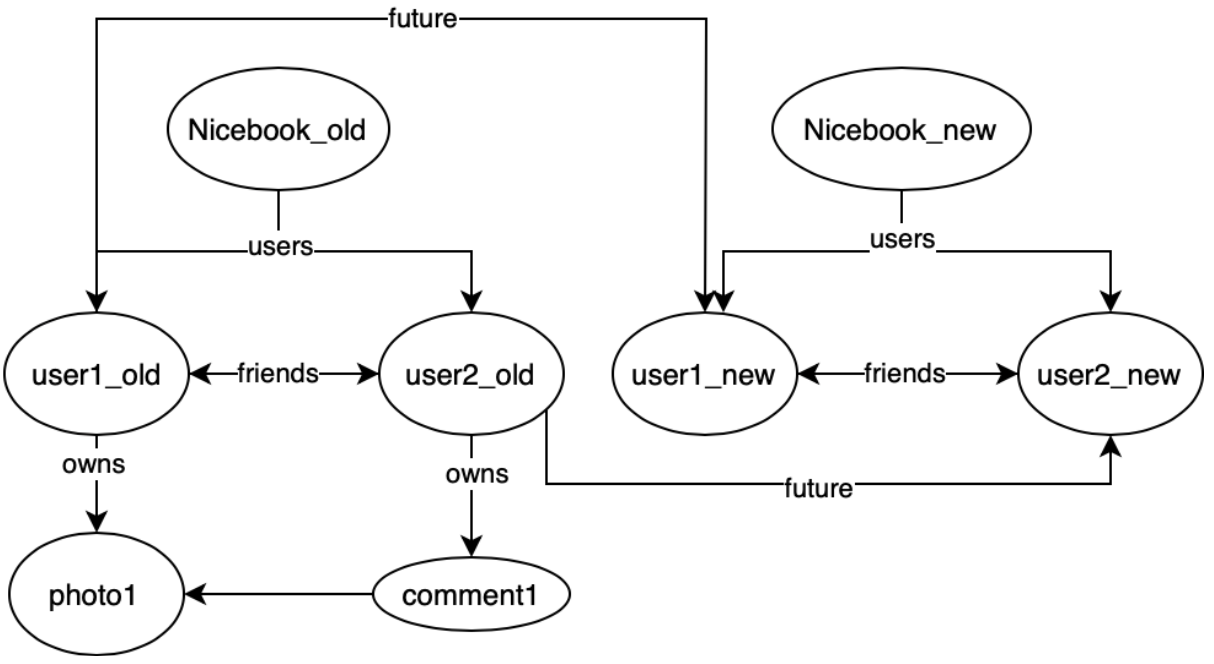
\includegraphics[width=6in]{images/modeling_decision_2.png}

	      We chose not to complicate our model by adding extra relations and went for option (b), where we only need to copy the content owner to the new Nicebook state, as shown below.

	      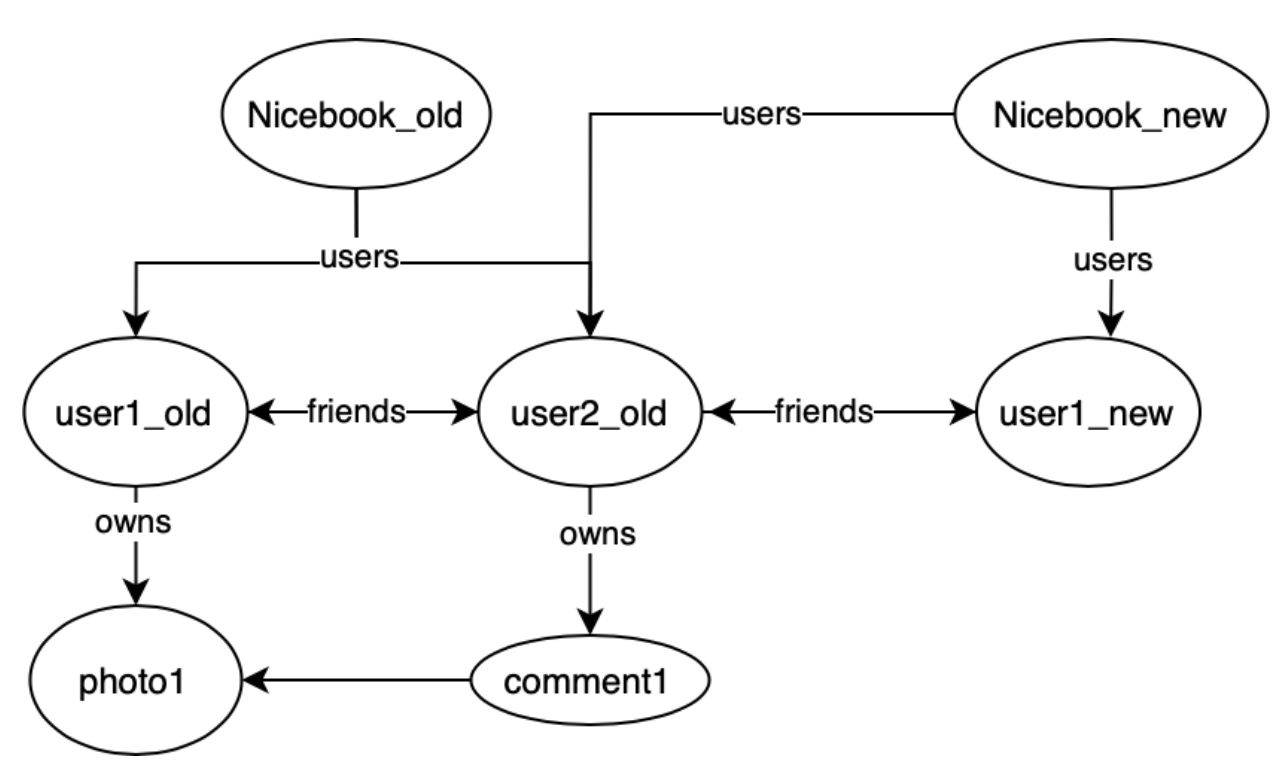
\includegraphics[width=6in]{images/modeling_decision_3.png}

	      Note that here it’s possible to reach the deleted photo1 from the new Nicebook state, but as we mentioned earlier, we will make it impossible for any user of the new state to view it (see function getContentsInState). Therefore, from a user’s point of view, virtually there’s no difference. We decided to follow this strategy for Tags as well.

	\item \textbf{Users can belong to multiple Nicebooks}\\
	      Following the deletion design, we allowed users to belong to multiple states. This is because, when we use an action to change a specific user’s state, it is difficult to change all the related user states.

	      For example, in the following diagram. We apply addPhoto action to user1, so user1 will be user1 and change its state. However, user1 has a friend relationship. The issue we face is how we maintain the relationship with the new user. We cannot create a new state for all users with a relationship with user1, like user2.

	      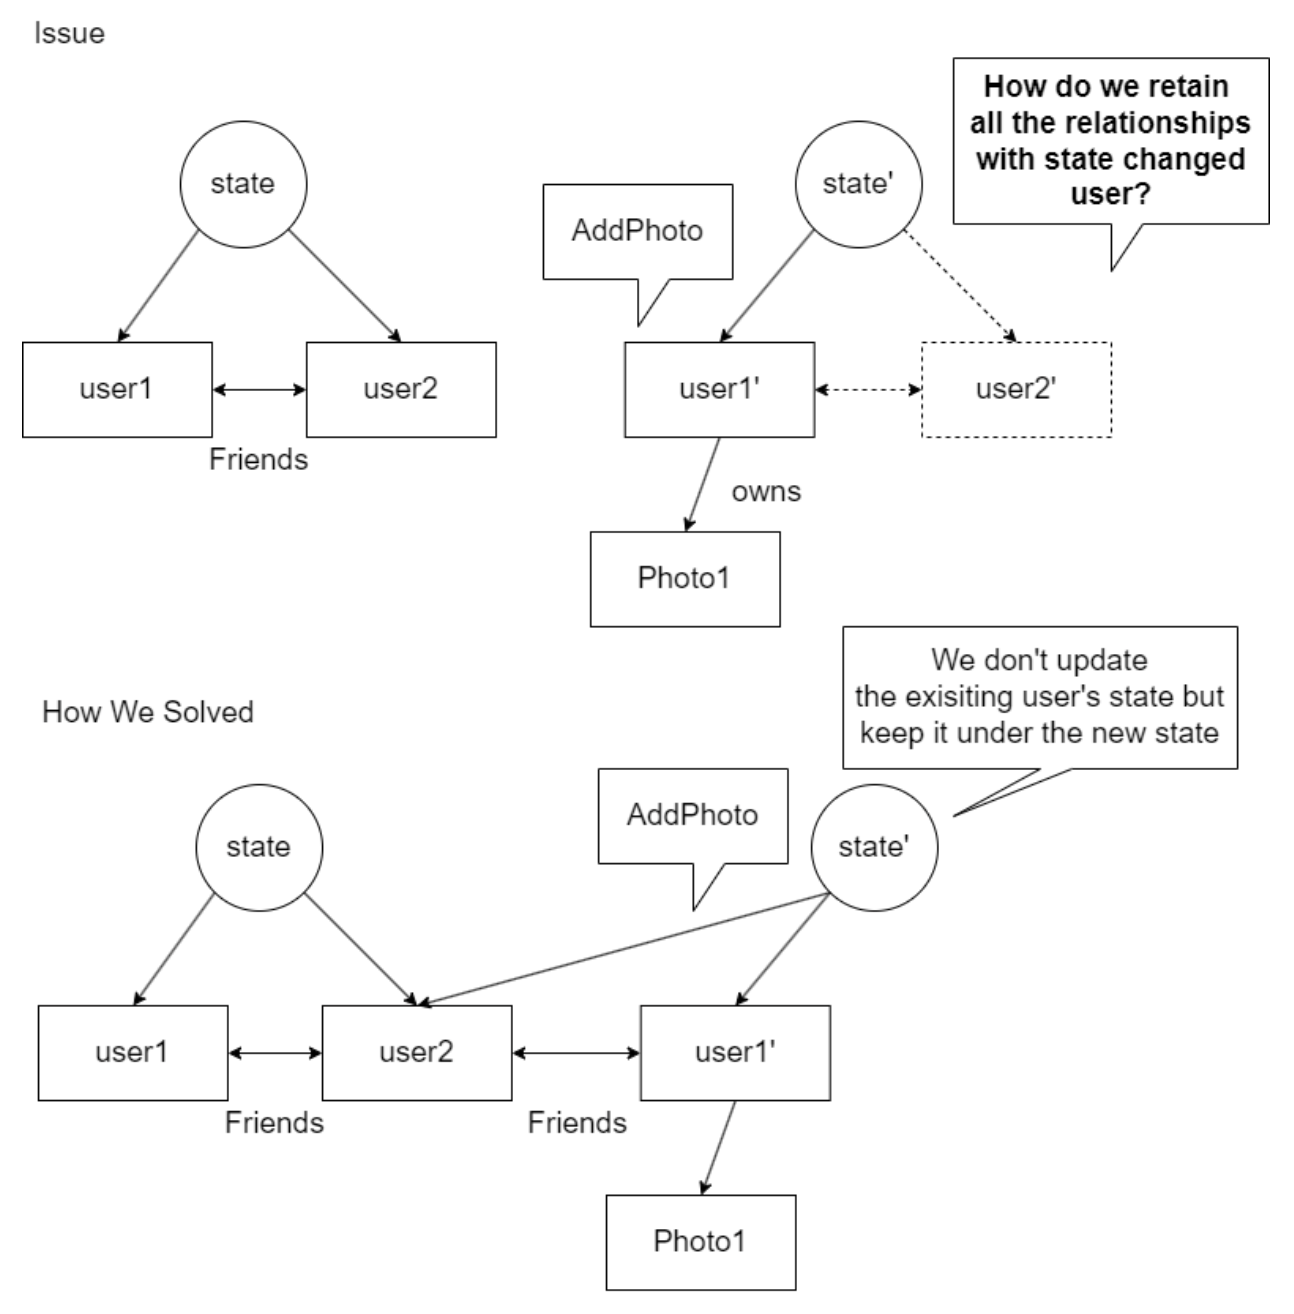
\includegraphics[width=6in]{images/multiple_nicebooks.png}

	      To solve this problem and the one mentioned in the previous section, we must users to be able to belong to multiple states. In this case, user1’s friend user2 can belong to both the new and old states. Using this method, we simply update the main user’s or content’s state in each action, making it easier to implement actions. Leaving our canView to handle users belonging to multiple states, which we will explain in the next section.

	\item \textbf{canView Implementation}\\
	      Respecting the assumptions we made in the previous sections, we defined our canView function by combining the following rules:
	      \begin{enumerate}
		      \item To be able to view that content, the owner of that content must exist under that state
		            \begin{enumerate}
			            \item We can extract all the viewable content by tracing from the state to the users and its own contents
		            \end{enumerate}
		      \item Privacy settings
	      \end{enumerate}
	      In the following example, Photo1 is viewable from state1, but in state2 it is not viewable, because the owner doesn’t belong to state2.

	      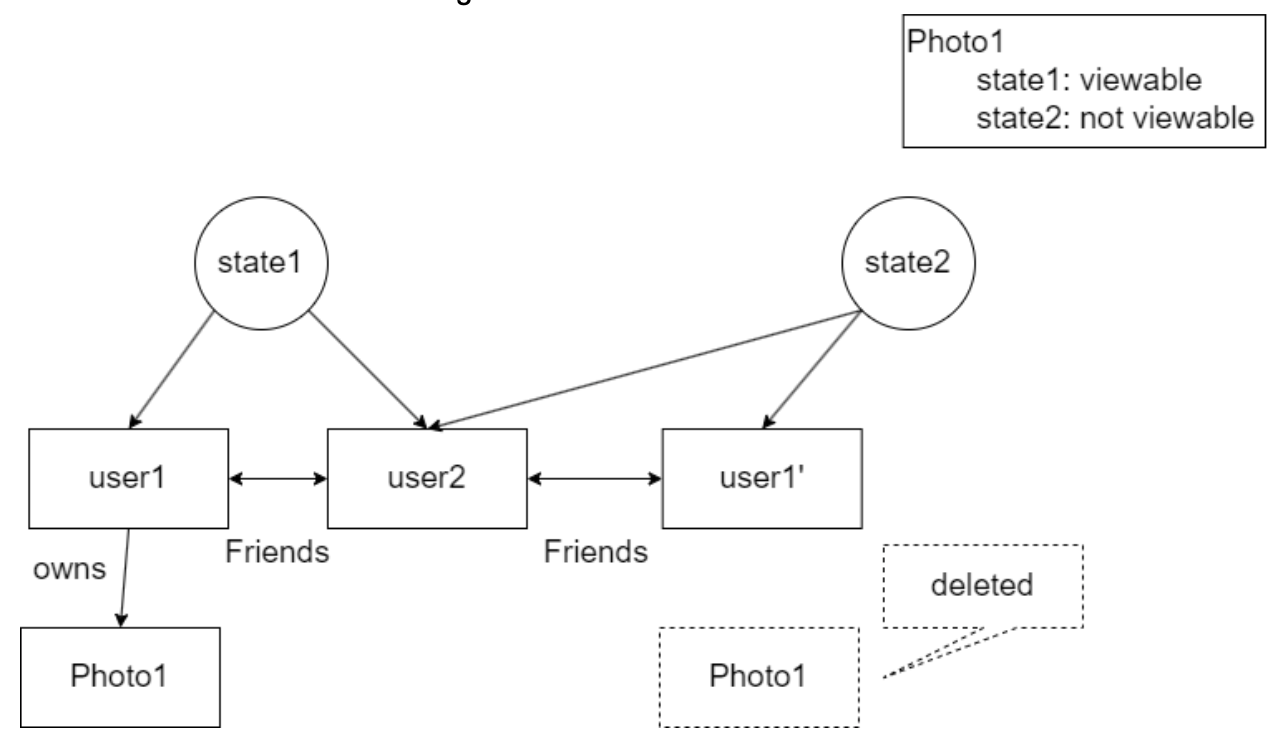
\includegraphics[width=6in]{images/canview.png}

	      We follow the same for tags. A Tag is viewable only if the tagged user exists in that state.
\end{enumerate}

\subsection{Describe any invariants that are not explicitly mentioned in the given document but were discovered during the modeling process.}
Following are the constraints and invariants that weren’t explicitly defined in the project specification but were discovered in the process
\begin{enumerate}
	\clearpage\item A nested comment chain cannot have cycles: A comment cannot be used to comment on itself or one of its “child” comments.

	      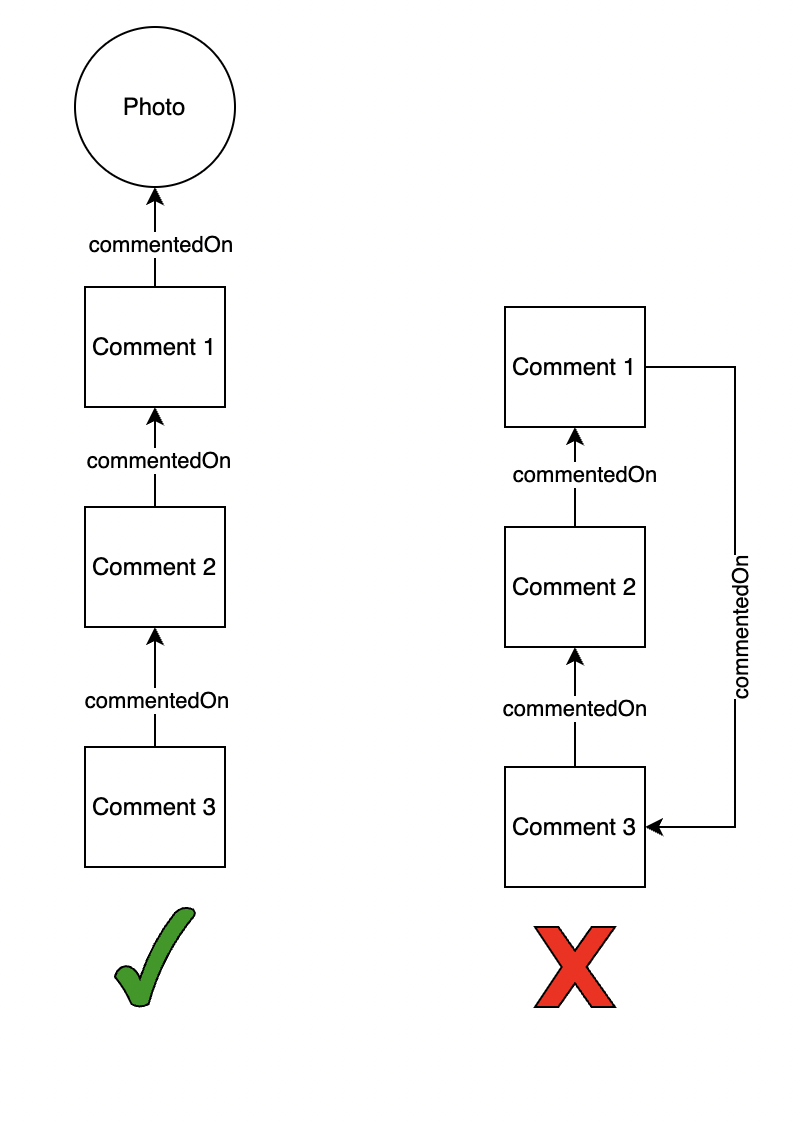
\includegraphics[width=5in]{images/invariant_1.png}

	      \clearpage\item A User cannot be friends with itself, however, loops in friendships are allowed.

	      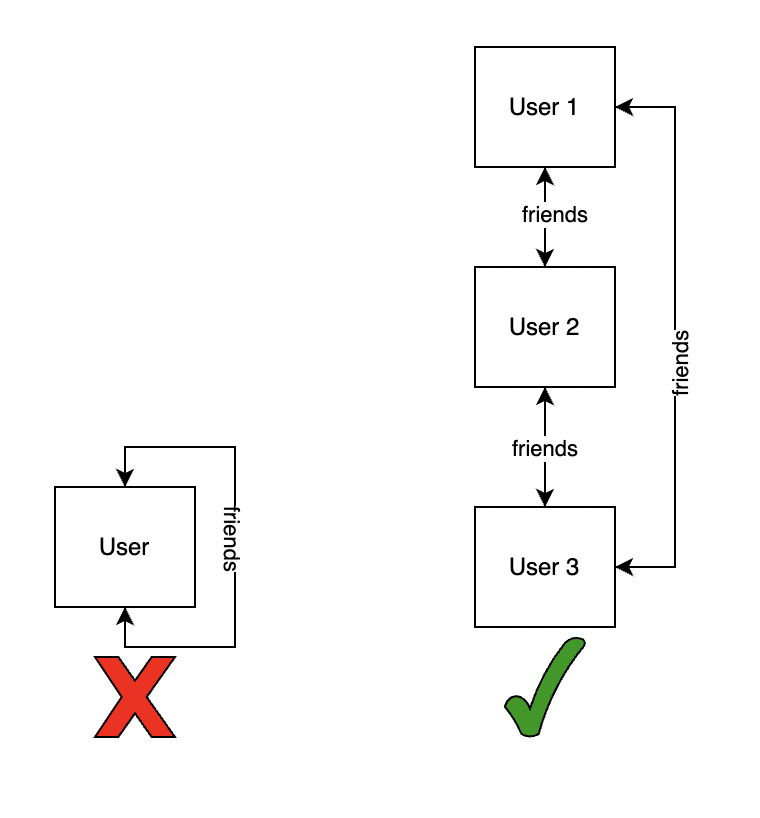
\includegraphics[width=5in]{images/invariant_2.png}

	      \clearpage\item Users can only be friends with users who share a state with the user.

	      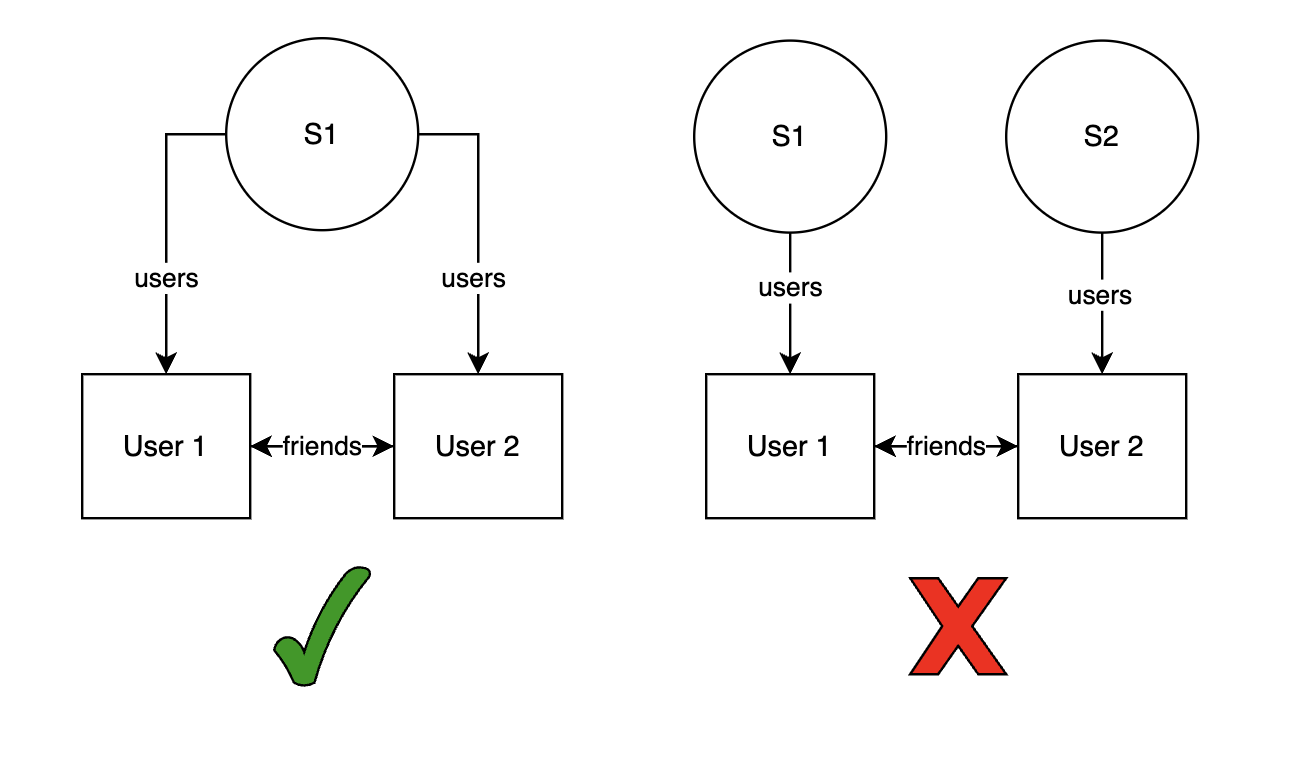
\includegraphics[width=5in]{images/invariant_3.png}

	      \clearpage\item A user cannot be tagged in the same photo by two different tag instances.

	      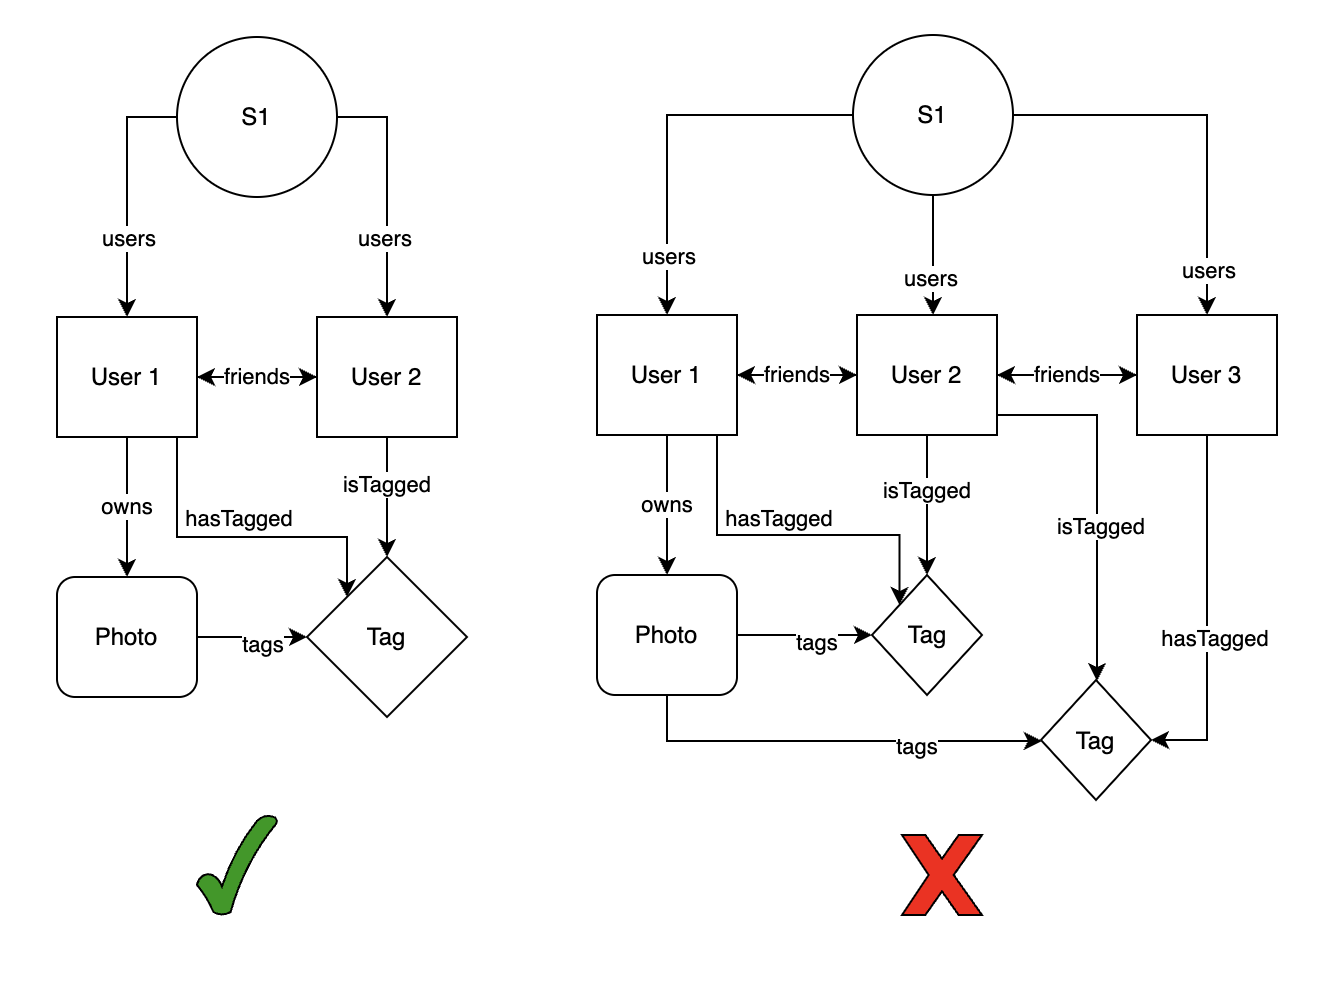
\includegraphics[width=5in]{images/invariant_4.png}

	      \clearpage\item Content should have exactly one owner in a state

	      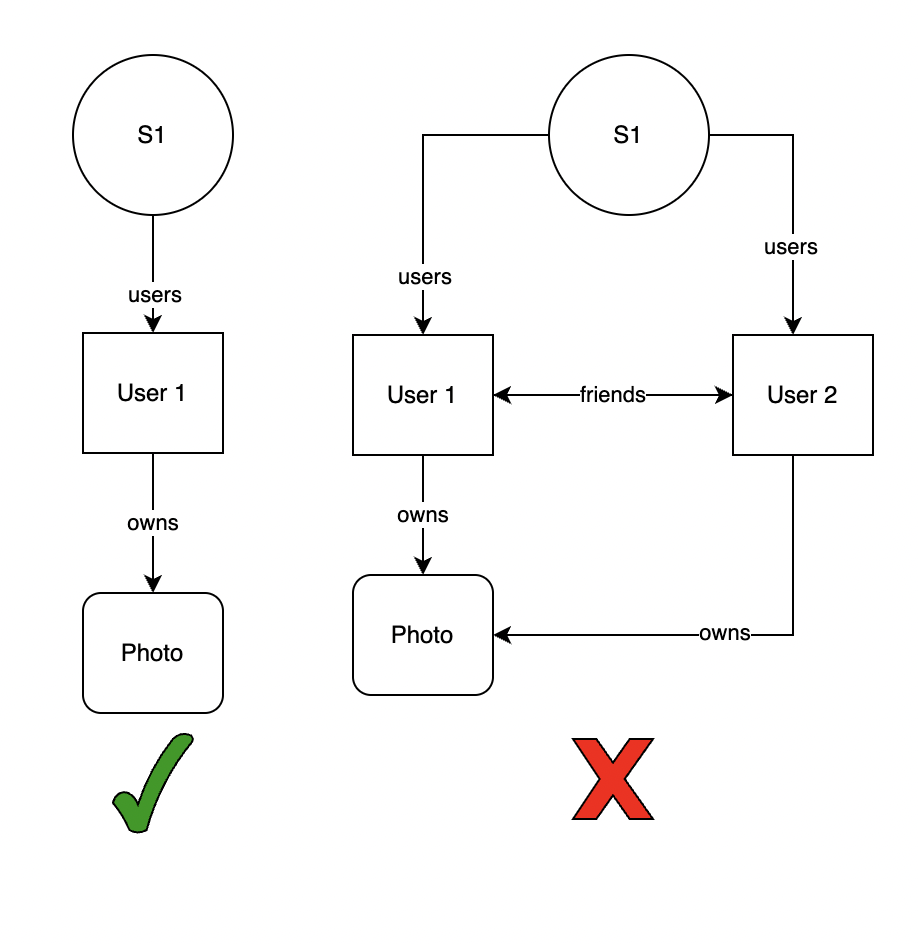
\includegraphics[width=5in]{images/invariant_5.png}

	      \clearpage\item A Tag instance should be mapped to exactly one pair of users in a state.

	      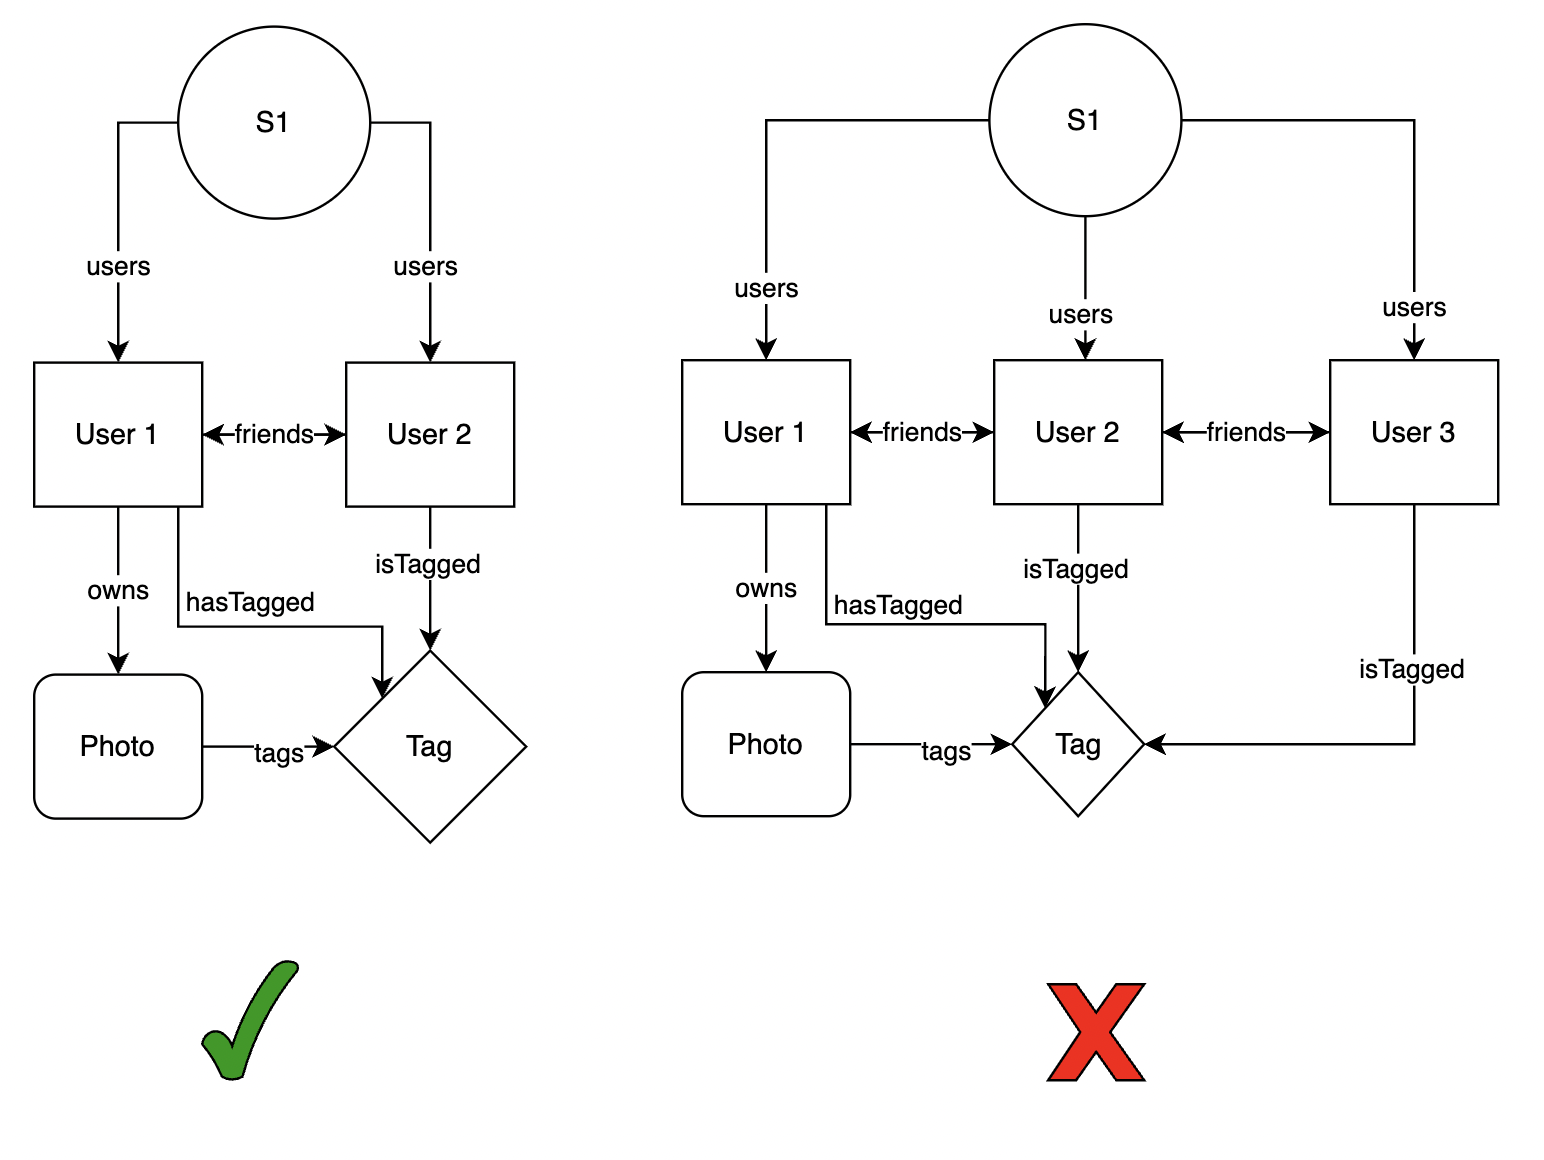
\includegraphics[width=5in]{images/invariant_6.png}

	\item While we check for commenting privileges and tagging privileges during operations that connect a pre-state and a post-state, we also must make sure that existing comments and tags satisfy the privileges that are required to add them. Therefore, as part of the invariants, we have defined two invariants: $invaraintNoCommentIsPresentWithoutPrivileges$ and $invariantNoTagIsPresentWithoutPrivileges$ that ensure that comments added are placed there in accordance with the privileges defined in canCommentOn, and the tags are existing on a photo where the the tagger and the tagged user are friends and the photo is viewable to both of them. In the diagram below, User C should not be able to comment on Comment 1 as it doesn’t even have the privilege to view Comment 1. Therefore the following is an invalid state.

	      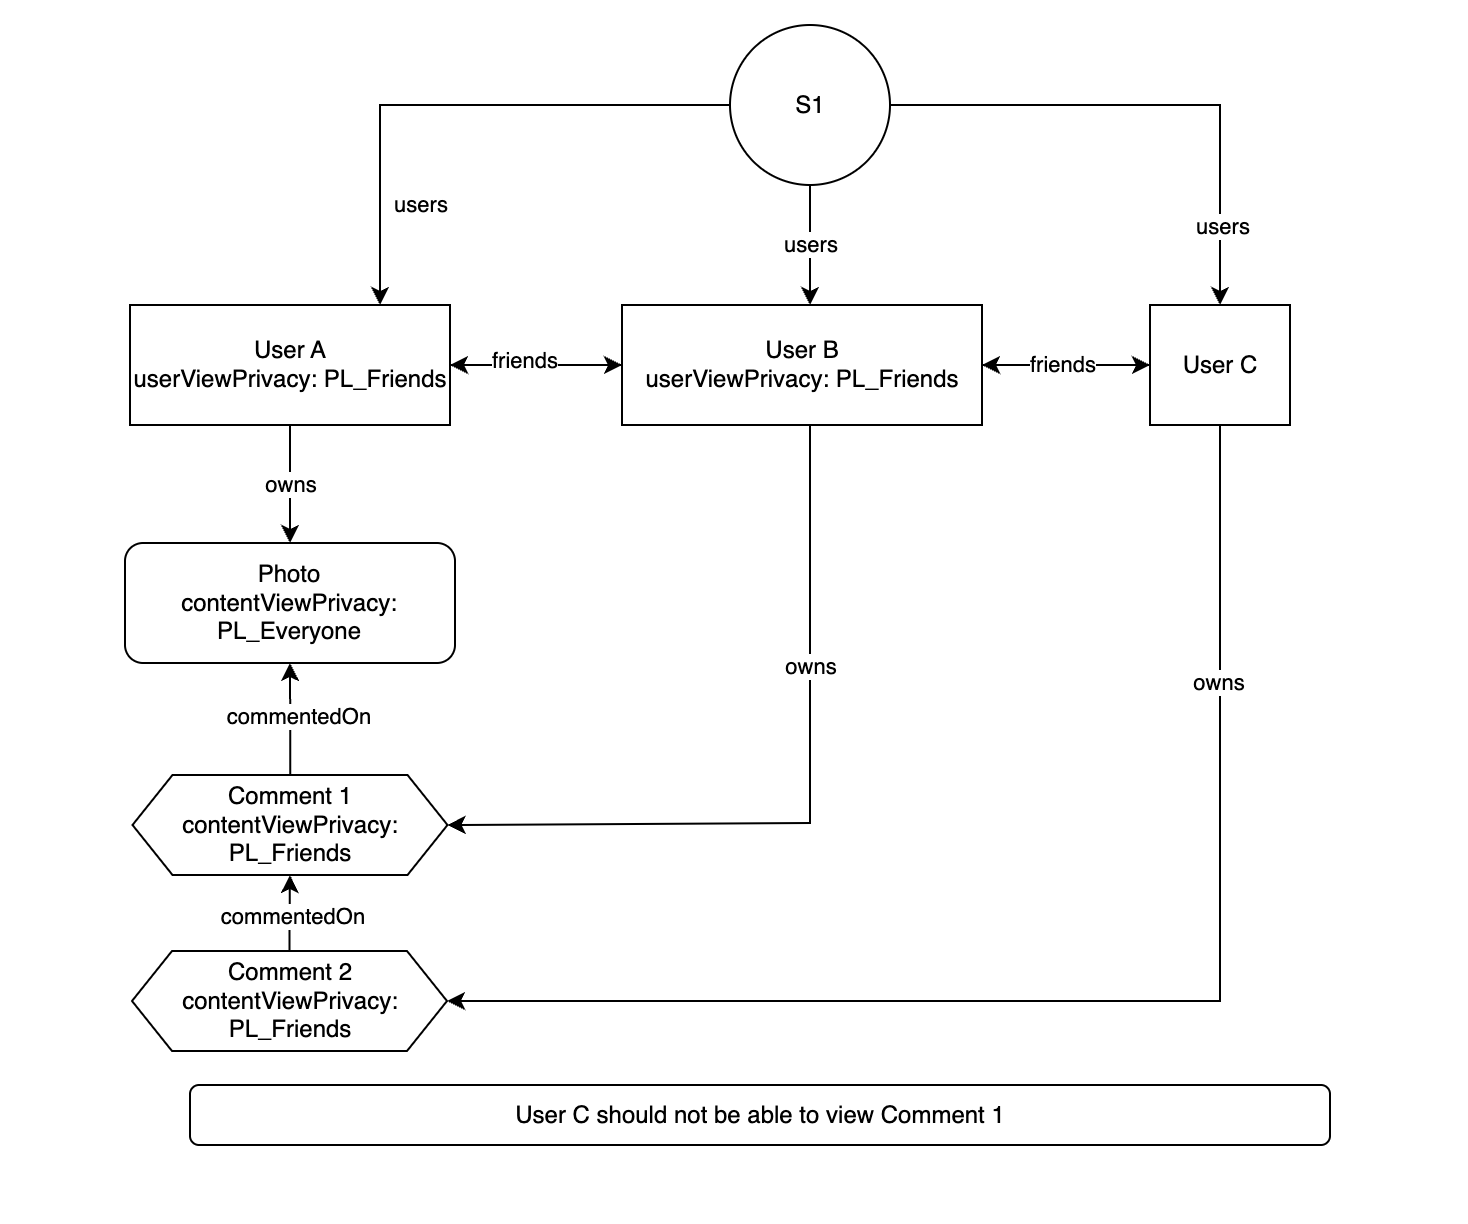
\includegraphics[width=6in]{images/invariant_7.png}
\end{enumerate}
\subsection{Describe an invariant that was violated by an operation in your model and how it was fixed.}
We defined an invariant named “invariantUserCanOnlyBeFriendsWithUsersInTheSameState
. This invariant defines that users cannot have a relationship with a friend in another state.\\

In addTag action, we defined two arguments: taggee who is a user to be tagged, and tagger who is a user to tag. In precondition, we declared that tagger should be tagged’s friend based on the spec, which said that “A user only tagged by its friends.”\\

At the first implementation, we changed only taggee’s state and promoted it as a new tagee because we designed how the system sees the tags in the current state as  “we can see the tag in the current state if and only if the tag has a tagged user that belongs to that state.” However, when we tried to generate instances, we noticed that this action doesn’t create any instances.\\

After some debugging, we found that addTag action violates “invariantUserCanOnlyBeFriendsWithUsersInTheSameState,” because we didn’t change the tagger’s state. Taggee is in the new state, but tagger is in the old state, but they are friends, which violates the invariant.\\

We fixed this problem by removing the invariant that constrained users to be friends with users of the same state. We then added a constraint that allows users to be friends with others who the user shares a state with.\\
\subsection{List the scope used for the analysis of invariant preservation. Why did you choose this scope, and why do you think it is sufficient?}

We have used the scope of 5 for the analysis of invariant preservation. We believe that the default scope, which is 3, was sometimes insufficient for representation actions such as removeTag or removePhoto, where we might want to 'copy' multiple objects to the new state. We wanted to ensure that alloy can comfortably generating instances when attempting to generate instances for checking Privacy Violations. The scope of 5 is sufficient for testing out our model, because none of our actions involve copying of more than two instances of an object, so 5 gives us more than enough room to test the cases which have multiple items linked to these items that are being copied.
\section{Task 2}
\subsection{Define an Alloy function called canView, which takes at least one parameter that represents some user in the
	social network, and returns the set of all content that can be viewed by that user. You may use any number of
	helper predicates or functions to define canView.}

See the alloy code we implemented.

\subsection{You will use canView to check whether it is possible for a user to access a piece of content against the intent of the owner. In particular, we say that a privacy violation has occurred if a user is able to view a piece of content without adhering to the privacy level that is assigned to the content by its owner. For example, suppose that Alice
	and Bob are not friends, and Alice has a photo that is assigned privacy setting Friends; if Bob is able to view the
	photo, this would be considered a privacy violation. Define an Alloy assertion called NoPrivacyViolation
	to check that no such violation is possible.}

See the alloy code we implemented.

\subsection{Does your model satisfy NoPrivacyViolation? If so, explain why. If not, include a counterexample that
	demonstrates a violation, and suggest a modification to the design of privacy settings in Nicebook. Describe
	any alternatives you considered and rejected, along with justifications for your decision.}

Our model satisfies NoPrivacyViolation. \\
In the model instance below, if User C is able to view the Comment owned by User B, this is a violation of NoPrivacyViolation Because of the following
\begin{itemize}
	\item The Comment's contentViewPrivacy is PL\_Friends and this allows User C to view he/she is friends with the owner of the Comment: User B.
	\item All parent elements of the Comment are also viewable to User C as the Photo's contentViewPrivacy is set to PL\_Everyone.
	\item However, User A has userViewPrivacy = PL\_Friends which only allows friends of User A to view comments on contents owned by User A. Since Comment is a comment on a Photo owned by User A, it should not be viewable to User C.
\end{itemize}

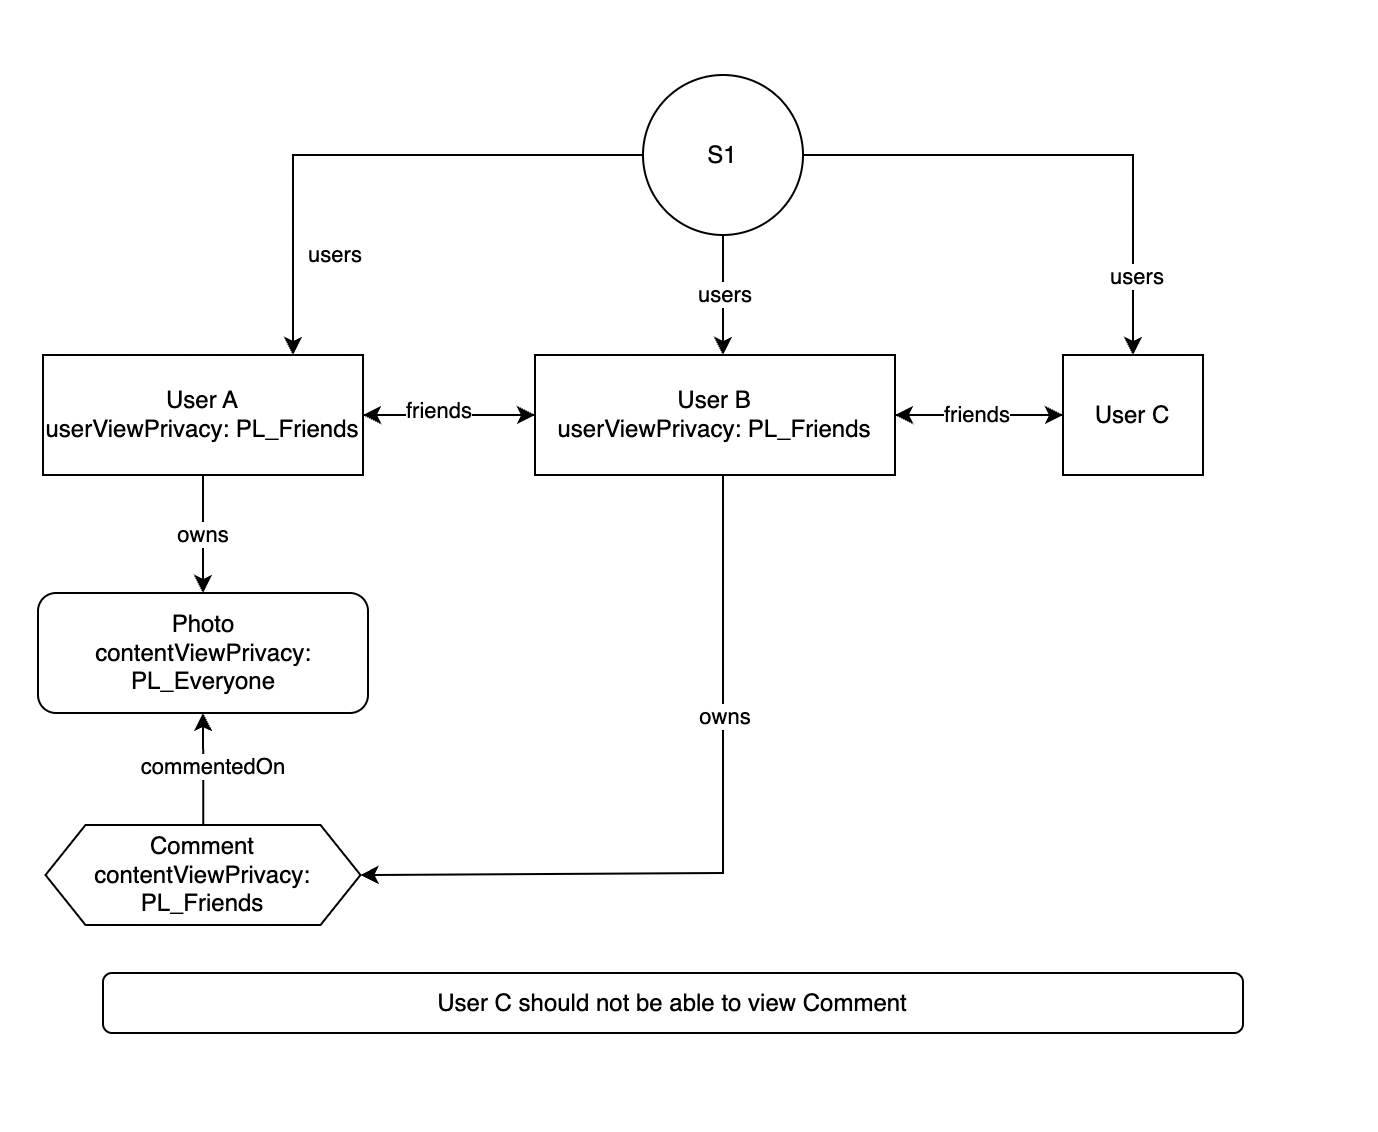
\includegraphics[width=6in]{images/privacy_violation.png}


\section{Task 3}
\subsection{What are the strengths and weaknesses of Alloy and its tool, the Alloy Analyzer?}
\subsubsection{Strengths of Alloy}
\begin{enumerate}
	\item \textbf{Powerful Relational Logic} \\
	      The most used operator in our project is the relational join. It is similar to the object oriented language but more powerful. For example, in java emp.dept.mng will return the manager of the department which the employee belongs to, while in alloy this will work even if the emp is a set of employees, dept is a set of departments and/or mng is a set of managers. Also, in Alloy we can navigate to the backward relation as well.
	\item \textbf{Powerful Model Design and Representation} \\
	      Alloy makes it easy to describe a universe of objects as a classification tree, with each relation defined over nodes in this tree. Which makes it easy to visualize the model and relation. Alloy Analyzer can generate a comprehensive graphical representation of the sets and relations from the signature declarations.
	\item \textbf{Limit Scope Analysis} \\
	      We can have a small scope that bounds each of the types in the specification. A scope of five, for example, would include tests involving at most five elements of each type.
	\item \textbf{Abstraction} \\
	      An abstract signature has no elements that do not belong to a child signature, and the extensions of a signature are disjoint.
\end{enumerate}
\subsubsection{Weaknesses of Alloy}
\begin{enumerate}
	\item \textbf{Ambiguity in the Inconsistency Error} \\
	      When there is an inconsistency error, Alloy does not specify where its section or line of code is, which makes it too hard to figure out the problem, especially when we work in a large system.
	\item \textbf{There is a Chance to Improve the Presentation of Different States} \\
	      Alloy is representing two different objects for the same signature, the first one presenting the current state and the other representing the post state. This leads to many issues in our project, but we handle this in our project by providing extra constraints and invariants related to states.
\end{enumerate}
\subsection{Under what situations would you recommend its use (or not)? Why?}
Software nowadays is involved in each and every aspect of our life. In communication, healthcare, transportation, airlines, agriculture, network, civil engineering, commerce, … and so on. So when designing a software system, we need to be able to express the structures essential to the design and to check that they have the properties we expect. If we checked the structure model manually, we couldn’t identify each behavior in the system. Using automated modeling tools like alloy is essential especially if the system is critical (and its minor bad state will result in huge impact)\\

We strongly recommend using alloy as a modeling tool. It is an easy and powerful language and shows its success in many huge projects. Alloy allows every possible behavior for the model, as we add constraints, the behavior is limited.

\subsection{With respect to this notation, what is the single most-important future development that would be needed to
	make it more generally useful to practitioners?}

Precise error trace specification for the inconsistency counter example. Refer to the first point in weaknesses of Alloy in the first question in Task 3.


\end{document}
